\chapter{Preliminaries}
\label{chap:preliminaries}

\chapterprecishere{%
  Maar ik maak steeds wat ik nog niet kan om het te leeren kunnen.\par\raggedleft---
  \textup{Vincent van Gogh}, The Complete Letters of Vincent Van Gogh, Volume Three}

Foundamental concepts in data science come from a variety of fields, including
mathematics, statistics, computer science, optimization theory, and information theory.
This chapter provides a brief overview of the main computational, mathematical and statistical
concepts in data science.

The goal is not to provide a comprehensive treatment of these topics, but to consolidate
notations and definitions that are used throughout the book.  The reader is encouraged to
consult the references provided at the end of each topic for a more in-depth treatment.
Statisticians with strong programming background and computer scientists with strong
statistics background will probably not find much new here.

I first introduce the main concepts in algorithms and data structures, which are the
building blocks of computational thinking.  Then, I present the basic concepts in set
theory and linear algebra, which are important mathematical foundations for data science.
Finally, I introduce the main concepts in probability theory, the cornerstone of
statistical learning and inference.

If your are familiar with these topics, you can safely skip this chapter.  Otherwise, I
encourage you to read it carefully, as it will help you understand the rest of the book.

\begin{mainbox}{Chapter remarks}

  \boxsubtitle{Contents}

  \startcontents[chapters]
  \printcontents[chapters]{}{1}{}
  \vspace{1em}

  \boxsubtitle{Context}

  \begin{itemize}
    \item Data science relies on a variety of mathematical and computational concepts.
    \item The main concepts are algorithms, data structures, set theory, linear algebra,
      and probability theory.
  \end{itemize}

  \boxsubtitle{Objectives}

  \begin{itemize}
    \item Introduce a brief overview of the main computational, mathematical and
      statistical concepts in data science.
    \item Remind the reader the main definitions and properties of these concepts.
    \item Consolidate notations and definitions that are used throughout the book.
  \end{itemize}
\end{mainbox}

{}
\clearpage

\section{Algorithms and data structures}

Algorithms are step-by-step procedures for solving a problem.  They are used to
manipulate data structures, which are ways of organizing data to solve problems.
They are realized in programming languages, which are formal languages that can be used
to express algorithms.

My suggestion of a comprehensive book about algorithms and data structures is
\textcite{Cormen2022}\footfullcite{Cormen2022}.

\subsection{Computational complexity}

The computational complexity of an algorithm is the amount of resources it uses to
run as a function of the size of the input.  The most common resources are time and
space.

Usually, we are interested in the asymptotic complexity of an algorithm, i.e. how
the complexity grows as the size of the input grows.  The most common notation for
asymptotic complexity is the Big-O notation.

\paragraph{Big-O notation}  Let $f$ and $g$ be functions from the set of natural numbers
to the set of real numbers, i.e. $f, g : \mathbb{N} \rightarrow \mathbb{R}$.  We say that $f$ is
$O(g)$ if there exists a constant $c > 0$ such that $f(n) \leq c g(n)$ for all $n \geq
n_0$, where $n_0$ is a natural number.
We can order functions by their asymptotic complexity.  For example, $O(1) < O(\log n) <
O(n) < O(n \log n) < O(n^2) < O(2^n) < O(n!)$\footnote{Throughout this book, we consider
$\log n = \log_2 n$.}.

The asymptotic analysis of algorithms is usually done in the worst-case scenario, i.e.
the maximum amount of resources the algorithm uses for any input of size $n$.  Thus,
it gives us an upper bound on the complexity of the algorithm.  In other words, an
algorithm with complexity $O(g(n))$ is guaranteed to run in at most $c g(n)$ time for some
constant $c$.

It does not mean, for instance, that an algorithm with time complexity $O(n)$ will always run
faster than an algorithm with time complexity $O(n^2)$, but that the former will run faster
for a large enough input size.

An important property of the Big-O notation is that
\[
  O(f) + O(g) = O(\max(f, g))\text{,}
\]
i.e. if an algorithm has two sequential steps with time complexity $O(f)$ and $O(g)$, the
highest complexity is the one that determines the overall complexity.

\subsection{Algoritmic paradigms}

Some programming techniques are used to solve a wide variety of problems.  They are called
algorithmic paradigms.  The most common ones are listed below.

\paragraph{Divide and conquer}  The problem is divided into smaller subproblems that are
solved recursively.  The solutions to the subproblems are then combined to give a solution
to the original problem.  Some example algorithms are merge sort, quick sort, and binary
search.

\begin{algobox}[label=alg:bsearch]{Binary search algorithm.}
  \KwData{A sorted array $\vec{a} = \left[a_1, a_2, \dots, a_n\right]$ and a key $x$}
  \KwResult{True if $x$ is in $\vec{a}$, false otherwise}
  $l \gets 1$\;
  $r \gets n$\;
  \While{$l \leq r$}{
    $m \gets \left\lfloor \frac{l + r}{2} \right\rfloor$\;
    \If{$x = a_m$}{
      \Return{\emph{true}}
    }
    \eIf{$x < a_m$}{
      $r \gets m - 1$\;
    }{
      $l \gets m + 1$\;
    }
  }
  \Return{\emph{false}}
  \tcblower
  An iterative algorithm that searches for a key in a sorted array.
\end{algobox}

Consider as an example the \cref{alg:bsearch} that solves the binary search problem.  Given a
$n$-elements sorted array $\vec{a} = \left[a_1, a_2, \dots, a_n\right]$, $a_1 \leq a_2 \leq
\dots \leq a_n$, and a key $x$, the algorithm returns true if $x$ is in $A$ and false
otherwise.  The algorithm works by dividing the array in half at each step and comparing
the key with the middle element.  Each time the key is not found, the search space is
reduced by half.

\begin{algobox}[label=alg:bsearch2]{Recursive binary search algorithm.}
  \SetKwProg{Fn}{function}{ is}{end}
  \Fn{$\operatorname{bsearch}(\left[a_1, a_2, \dots, a_n\right], x)$}{
    \If{$n = 0$}{
      \Return{\emph{false}}
    }
    $m \gets \left\lfloor \frac{n}{2} \right\rfloor$\;
    \If{$x = a_m$}{
      \Return{\emph{true}}
    }
    \eIf{$x < a_m$}{
      \Return{$\operatorname{bsearch}(\left[a_1, \dots, a_{m-1}\right], x)$}
    }{
      \Return{$\operatorname{bsearch}(\left[a_{m+1}, \dots, a_{n}\right], x)$}
    }
  }
  \tcblower
  A recursive algorithm that searches for a key in a sorted array.  Note that trivial
  conditions --- $n = 0$ and key found --- are handled first, so the recursion stops
  when the problem is small enough.
\end{algobox}

Divide and conquer algorithms can be implemented using recursion.  \emph{Recursion}
is also a algorithmic paradigm where a function calls itself to solve smaller instances of the
same problem.  The recursion stops when the problem is small enough to be solved directly.

\Cref{alg:bsearch2} shows a recursive implementation of the binary search algorithm.
The smaller instances, or so called \emph{base cases}, are when the array is empty or the key
is found in the middle.  Other conditions --- key is smaller or greater than the middle element ---
are handled by calling the function recursively with the left or right half of the array.

% \paragraph{Dynamic programming}  The problem is divided into overlapping subproblems, and
% the solutions to the subproblems are only solved once. The subproblems are then optimized
% to find the overall solution.  Some example algorithms are the Bellman-Ford algorithm,
% Floyd-Warshall algorithm, and the Knapsack problem.

This solution --- both algorithms --- has a worst-case time complexity of $O(\log n)$. The
search space is halved at each step, thus, in the $i$-th iteration, the remaining number
of elements in the array is $n / 2^{i-1}$.  In the worst-case, the algorithm stops when the
search space has size $1$ or smaller, i.e.
\[
  \frac{n}{2^{i-1}} = 1 \implies
  i = 1 + \log n\text{.}
\]

Note this strategy leads to such a low time complexity that we can solve large instances
of the problem in a reasonable amount of time.  Consider the case of an array with $2^{64}
= 18{,}446{,}744{,}073{,}709{,}551{,}616$ elements, the algorithm will find the key in at most $65$
steps.

\clearpage
\paragraph{Greedy algorithms}  The problem is solved with incremental steps, each of which
is locally optimal.  The overall solution is not guaranteed to (but might) be optimal.  Some example
algorithms are Dijkstra's algorithm and Prim's algorithm.  Greedy algorithm are usually
very efficient in terms of time complexity --- see more in the following.

One example of suboptimal greedy algorithm is a heuristic solution for the knapsack problem.
The \emph{knapsack problem} is a combinatorial optimization problem where the goal is to
maximize the value of items in a knapsack without exceeding its capacity.  The problem is
mathematically defined as
\[
  \text{maximize }~\sum_{i = 1}^n v_i x_i\text{,}
\]
\[
  \text{subject to }~\sum_{i = 1}^n w_i x_i \leq W\text{,}
\]
where $v_i$ is the value of item $i$, $w_i$ is the weight of item $i$, $x_i$ is a binary
variable that indicates if item $i$ is in the knapsack, and $W$ is the capacity of the
knapsack.

\begin{algobox}[label=alg:knapsack]{Heuristic solution for the knapsack problem.}
  \KwData{A list of $n$ items, each with a value $v_i$ and a weight $w_i$, and a capacity $W$}
  \KwResult{The binary variable $x_i$ for each item $i$ that maximizes the total value}
  Sort the items in decreasing order of value\;
  $V \gets 0$\;
  $x_i \gets 0,~\forall i$\;
  \For{$i \gets 1$ \KwTo $n$}{
    \If{$w_i \leq W$}{
      $x_i \gets 1$\;
      $V \gets V + v_i$\;
      $W \gets W - w_i$\;
    }
  }
  \Return{$x_i,~\forall i$}
  \tcblower
  A greedy algorithm that solves suboptimally the knapsack problem.  The algorithm iterates over
  the items in decreasing order of value and puts the item in the knapsack if it fits.
\end{algobox}

An algorithm that finds a suboptimal solution for the knapsack problem is shown in
\cref{alg:knapsack}.
It iterates over the items in decreasing order of value and puts the item in the
knapsack if it fits.  The algorithm is suboptimal because there might exist small-value
items that, when combined, would fit in the knapsack and yield a higher total value.

The most costly operation in the algorithm is the sorting of the items in
decreasing order of value, which has a time complexity\footnote{%
Considering the worst-case time complexity of the sorting algorithm, consult
\fullcite{Cormen2022} for more details.} of $O(n \log n)$.

\paragraph{Brute force}  The problem is solved by trying all possible solutions.  Most of
the time, brute force algorithms have exponential time complexity, leading to impractical
solutions for large instances of the problem.  On the other hand, brute force algorithms
are usually easy to implement and understand, as well as guaranteed to find the optimal
solution.

In the previous example, a brute force algorithm for the knapsack problem would
try all possible combinations of items and select the one that maximizes the total value
without exceeding the capacity.  One can easily see that the time complexity of such an
algorithm is $O(2^n)$, where $n$ is the number of items, as there are $2^n$ possible
combinations of items.  Such an \emph{exhaustive search} is impractical for large $n$,
but it is guaranteed to find the optimal solution.

One should avoid brute force algorithms whenever possible, as they are usually too costly
to be practical.  However, they are useful for small instances of the problem, for
verification of the results of other algorithms, and for educational purposes.

\paragraph{Backtracking}  The problem is solved incrementally, one piece at a time.  If a
piece does not fit, it is removed and replaced by another piece.  Some example algorithms
are the naïve solutions for N-queens problem and for the Sudoku problem.  Backtracking, as
a special case of brute force, often leads to exponential (or worse) time complexity.

Many times, backtracking algorithms are combined with other techniques to reduce the
search space and make the algorithm more efficient.  For example, the backtracking
algorithm for the Sudoku problem is combined with constraint propagation to reduce the
number of possible solutions.

\clearpage
A Sudoku puzzle consists of an $n \times n$ grid, divided into $n$ subgrids of size
$\sqrt{n} \times \sqrt{n}$.  The goal is to fill the grid with numbers from $1$ to $n$
such that each row, each column, and each subgrid contains all numbers from $1$ to $n$ but
no repetitions.  The most common grid size is $9 \times 9$.

\begin{figurebox}[label=fig:sudoku]{Backtracking to solve a Sudoku puzzle.}
  \centering
  \begin{tikzpicture}
    % a tree like structure with the Sudoku puzzle at the root, and tries to fill each cell
    % with a number, backtracking when a number does not fit

    % an almost complete Sudoku puzzle
    \node (root) at (1, 0) {$\begin{array} {|c|c|c|c|}
      \hline
      ? &   &   & 1 \\
      \hline
      1 & 2 & 4 &   \\
      \hline
        & 4 & 1 & 2 \\
      \hline
      2 &   &   &   \\
      \hline
      \end{array}$};
    % node with first cell filled with 1
    \node (n1) at (-3.6, -3) {$\begin{array} {|c|c|c|c|}
      \hline
      \color{gray} 1 &   &   & \color{gray} 1 \\
      \hline
      \color{gray} 1 & 2 & 4 &   \\
      \hline
        & 4 & 1 & 2 \\
      \hline
      2 &   &   &   \\
      \hline
      \end{array}$};
    % node with first cell filled with 2
    \node (n2) at (-1.2, -3) {$\begin{array} {|c|c|c|c|}
      \hline
      \color{gray} 2  &   &   & 1 \\
      \hline
      1 & \color{gray} 2 & 4 &   \\
      \hline
        & 4 & 1 & 2 \\
      \hline
      \color{gray} 2 &   &   &   \\
      \hline
      \end{array}$};
    % node with first cell filled with 3
    \node (n3) at (1.2, -5) {$\begin{array} {|c|c|c|c|}
      \hline
      3  & ? &   & 1 \\
      \hline
      1 & 2 & 4 &   \\
      \hline
        & 4 & 1 & 2 \\
      \hline
      2 &   &   &   \\
      \hline
      \end{array}$};
    % node with first cell filled with 4
    \node (n4) at (3.6, -3) {$\begin{array} {|c|c|c|c|}
      \hline
      4  & ?  &   & 1 \\
      \hline
      1 & 2 & 4 &   \\
      \hline
        & 4 & 1 & 2 \\
      \hline
      2 &   &   &   \\
      \hline
      \end{array}$};
    % node with the second cell filled with 1
    \node (n5) at (-3.6, -8) {$\begin{array} {|c|c|c|c|}
      \hline
      3 & \color{gray} 1 &   & \color{gray} 1 \\
      \hline
      \color{gray} 1 & 2 & 4 &   \\
      \hline
        & 4 & 1 & 2 \\
      \hline
      2 &   &   &   \\
      \hline
      \end{array}$};
    % node with the second cell filled with 2
    \node (n6) at (-1.2, -8) {$\begin{array} {|c|c|c|c|}
      \hline
      3 & \color{gray} 2 &   & 1 \\
      \hline
      1 & \color{gray} 2 & 4 &   \\
      \hline
        & 4 & 1 & 2 \\
      \hline
      2 &   &   &   \\
      \hline
      \end{array}$};
    % node with the second cell filled with 3
    \node (n7) at (1.2, -8) {$\begin{array} {|c|c|c|c|}
      \hline
      \color{gray} 3 & \color{gray} 3 &   & 1 \\
      \hline
      1 & 2 & 4 &   \\
      \hline
        & 4 & 1 & 2 \\
      \hline
      2 &   &   &   \\
      \hline
      \end{array}$};
    % node with the second cell filled with 4
    \node (n8) at (3.6, -8) {$\begin{array} {|c|c|c|c|}
      \hline
      3 & \color{gray} 4 &   & 1 \\
      \hline
      1 & 2 & 4 &   \\
      \hline
        & \color{gray} 4 & 1 & 2 \\
      \hline
      2 &   &   &   \\
      \hline
      \end{array}$};
    % etc
    \node (dots) at (3.6, -5) {\dots};
    % arrows
    \draw[-Stealth] (root.west) -- (n1.north);
    \draw[-Stealth] (n1.north) -- (root.south west);
    \draw[-Stealth] (root.south west) -- (n2.north);
    \draw[-Stealth] (n2.north) -- (root.south);
    \draw[-Stealth] (root.south) -- (n3.north west);

    \draw[-Stealth] (n3.north west) -- (n5.north);
    \draw[-Stealth] (n5.north) -- (n3.south west);
    \draw[-Stealth] (n3.south west) -- (n6.north);
    \draw[-Stealth] (n6.north) -- (n3.south);
    \draw[-Stealth] (n3.south) -- (n7.north);
    \draw[-Stealth] (n7.north) -- (n3.south east);
    \draw[-Stealth] (n3.south east) -- (n8.north);
    \draw[-Stealth] (n8.north) -- (n3.north east);

    \draw[-Stealth] (n3.north east) -- (root.south east);
    \draw[-Stealth] (root.south east) -- (n4.north);

    \draw[-Stealth] (n4.south) -- (dots);
  \end{tikzpicture}
  \tcblower
  A Sudoku puzzle --- in this case, $4 \times 4$ --- is solved by trying all possible
  numbers in each cell and backtracking when a number does not fit.  The solution is found
  when all cells are filled and the constraints are satisfied.  Arrows indicate the
  backtracking steps.  The question mark indicates an empty cell that needs to be filled
  at that step.  Constraints violation are shown in gray.
\end{figurebox}

An illustration of backtracking to solve a $4 \times 4$ Sudoku puzzle\footnote{%
Smaller puzzles are more didactic, but the same principles apply to larger puzzles.}
is shown in \cref{fig:sudoku}.
The puzzle is solved by trying all possible numbers in each cell and backtracking when a
number does not fit.  The solution is found when all cells are filled and the constraints
are satisfied.  Arrows indicate the the steps of the backtracking algorithm.  Every time a
constraint is violated --- indicated in gray ---, the algorithm backtracks to the previous
cell and tries a different number.

One can easily see that a puzzle with $m$ missing cells has $n^m$ possible solutions.  For
small values of $m$ and $n$, the algorithm is practical, but for large values, it becomes
too costly.

\subsection{Data structures}

Data structures are ways of organizing data to solve problems.  The most common ones
are listed below.  A comprehensive material about the properties and implementations of
data structures can be found in \textcite{Cormen2022}\footfullcite{Cormen2022}.

\paragraph{Arrays}  An array is a homogeneous collection of elements that are accessed by
an integer index.  The elements are usually stored in contiguous memory locations.
In the scope of this book, it is equivalent to a mathematical vector whose element's type
are not necessarily numerical.  Thus, a $n$-elements array $\vec{a}$ is denoted by
$\left[a_1, a_2, \dots, a_n\right]$, where the $i$ in $a_i$ is the index of the element.

% \paragraph{Linked lists}  A linked list is a collection of elements called nodes.  Each
% node contains a value and a pointer to the next node in the list.  The first node is
% called the head, and the last node is called the tail.  The tail points to a null
% reference.

\paragraph{Stacks}  A stack is a collection of elements that are accessed in a
last-in-first-out (LIFO) order.  Elements are added to the top of the stack and
removed from the top of the stack.  In other words, only two operations are
allowed: push (add an element to the top of the stack) and pop (remove the top element).
Only the top element is accessible.

\paragraph{Queues}  A queue is a collection of elements that are accessed in a
first-in-first-out (FIFO) order.  Elements are added to the back of the queue and
removed from the front of the queue.  The two operations allowed are enqueue (add an
element to the back of the queue) and dequeue (remove the front element).  Only the
front and back elements are accessible.

\paragraph{Trees}  A tree is a collection of nodes.  Each node contains a value and a list
of references to its children.  The first node is called the root.  A node with no
children is called a leaf.  No cycles are allowed in a tree, i.e. a child cannot be an
ancestor of its parent. The most common type of tree is the binary tree, where each node
has at most two children.

Mathematically, a binary tree is a recursive data structure.  A binary tree is either
empty or consists of a root node and two binary trees, called the left and right
children.   Thus, a binary tree $T$ is
\[
  T = \begin{cases}
    \emptyset & \text{if it is empty, or} \\
    \left(v, T_l, T_r\right) & \text{if it has a value $v$ and two children $T_l$ and $T_r$.}
  \end{cases}
\]
Note that the left and right children are themselves binary trees.  If $T$ is a leaf,
then $T_l = T_r = \emptyset$.

This properties makes it easy to represent a binary tree using parentheses notation.  For
example, $(1, (2, \emptyset, \emptyset), (3, \emptyset, \emptyset))$ is a binary tree
with root $1$, left child $2$, and right child $3$.

\paragraph{Graphs}  A graph is also a collection of nodes.  Each node contains a value and a
list of references to its neighbors; the references are called edges.  A graph can be
directed or undirected.  A graph is directed if the edges have a direction.

Mathematically, a graph is a pair $G = (V, E)$, where $V$ is a set of vertices and $E \in
V \times V$ is a set of edges.  An edge is a pair of vertices, i.e. $e = (v_i, v_j)$,
where $v_i, v_j \in V$. If the graph is directed, the edge is an ordered pair, i.e. $e =
(v_i, v_j) \neq (v_j, v_i)$.

Not only each node can hold a value, but also each edge can have a weight.  A weighted
graph is a graph where there exists a function $w : E \rightarrow \mathbb{R}$ that assigns
a real number to each edge.

\begin{figurebox}[label=fig:graph]{A graph with four vertices and five edges.}
  \centering
  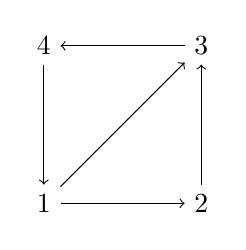
\begin{tikzpicture}
    % a graph with four vertices and five edges
    \node (v1) at (0, 0) {1};
    \node (v2) at (2, 0) {2};
    \node (v3) at (2, 2) {3};
    \node (v4) at (0, 2) {4};
    \draw[->] (v1) -- (v2);
    \draw[->] (v2) -- (v3);
    \draw[->] (v3) -- (v4);
    \draw[->] (v4) -- (v1);
    \draw[->] (v1) -- (v3);
  \end{tikzpicture}
  \tcblower
  A graph with four vertices and five edges.  Vertices are numbered from $1$ to $4$, and
  edges are represented by arrows.  The graph is directed, as the edges have a direction.
\end{figurebox}

A graphical representation of a directed graph with four vertices and five edges is shown
in \cref{fig:graph}.  The vertices are numbered from $1$ to $4$, and the edges are
represented by arrows.

Another common representation of a graph is the adjacency matrix.  An adjacency matrix is
a square matrix $A$ of size $n \times n$, where $n$ is the number of vertices.  The
$i, j$-th entry of the matrix is $1$ if there is an edge from vertex $i$ to vertex $j$,
and $0$ otherwise.  The adjacency matrix of the graph in \cref{fig:graph} is
\[
  A = \begin{pmatrix}
    0 & 1 & 1 & 0 \\
    0 & 0 & 1 & 0 \\
    0 & 0 & 0 & 1 \\
    1 & 0 & 0 & 0
  \end{pmatrix}\text{.}
\]

% \paragraph{Map} A map is a collection of key-value pairs.  The keys are unique, and
% each key is associated with a value.  The keys are used to access the values.

\section{Set theory}

A set is a collection of elements.  The elements of a set can be anything, including
other sets.  The elements of a set are unordered, and each element is unique.  The
most common notation for sets is the curly braces notation, e.g. $\{1, 2, 3\}$.

Some special sets are listed below.

\paragraph{Universe set}  The universe set is the set of all elements in a given context.
It is denoted by $\Omega$.

\paragraph{Empty set}  The empty set is the set with no elements.  It is denoted by
the symbol $\emptyset$.  Depending on the context, it can also be denoted by $\{\}$.

\subsection{Set operations}

The basic operations on sets are union, intersection, difference, and complement.

\paragraph{Union}  The union of two sets $A$ and $B$ is the set of elements that are in
$A$ or $B$.  It is denoted by $A \cup B$.  For example, the union of $\{1, 2, 3\}$ and
$\{3, 4, 5\}$ is $\{1, 2, 3, 4, 5\}$.

\paragraph{Intersection}  The intersection of two sets $A$ and $B$ is the set of elements
that are in both $A$ and $B$.  It is denoted by $A \cap B$.  For example, the intersection
of $\{1, 2, 3\}$ and $\{3, 4, 5\}$ is $\{3\}$.

\paragraph{Difference}  The difference of two sets $A$ and $B$ is the set of elements
that are in $A$ but not in $B$.  It is denoted by $A \setminus B$.  For example, the
difference of $\{1, 2, 3\}$ and $\{3, 4, 5\}$ is $\{1, 2\}$.

\paragraph{Complement}  The complement of a set $A$ is the set of elements that are not
in $A$.  It is denoted by $A^c = \Omega \setminus A$.

\paragraph{Inclusion}  Inclusion is a relation between sets.  A set $A$ is included in a
set $B$ if all elements of $A$ are also elements of $B$.  It is denoted by $A \subseteq B$.

\subsection{Set operations properties}

Union and intersection are commutative, associative and distributive.  Thus, given sets
$A$, $B$, and $C$, the following statements hold:
\begin{itemize}
  \item \emph{Commutativity:} $A \cup B = B \cup A$ and $A \cap B = B \cap A$;
  \item \emph{Associativity:} $(A \cup B) \cup C = A \cup (B \cup C)$ and $(A \cap B) \cap C = A \cap (B \cap C)$;
  \item \emph{Distributivity:} $A \cup (B \cap C) = (A \cup B) \cap (A \cup C)$ and $A \cap (B \cup C) = (A \cap B) \cup (A \cap C)$.
\end{itemize}

The difference operation can be expressed in terms of union and intersection as
\[
  A \setminus B = A \cap B^c\text{.}
\]

The complement of the union of two sets is the intersection of their complements, i.e.
\[
  (A \cup B)^c = A^c \cap B^c\text{.}
\]
Similarly, the complement of the intersection of two sets is the union of their complements, i.e.
\[
  (A \cap B)^c = A^c \cup B^c\text{.}
\]
This property is known as De Morgan's laws.

In terms of inclusion, given sets $A$, $B$, and $C$, the following statements hold:
\begin{itemize}
  \item \emph{Reflexity:} $A \subseteq A$;
  \item \emph{Antisymmetry:} $A \subseteq B$ and $B \subseteq A$ if and only if $A = B$;
  \item \emph{Transitivity:} $A \subseteq B$ and $B \subseteq C$ implies $A \subseteq C$.
\end{itemize}

\subsection{Relation to Boolean algebra}

Set operations are closely related to Boolean algebra.  In Boolean algebra, the elements
of a set are either true or false, many times represented by $1$ and $0$, respectively.
The union operation is equivalent to the logical OR operation, expressed by the symbol
$\lor$; and the intersection operation is equivalent to the logical AND operation,
expressed by the symbol $\land$.  The compliment operation is equivalent to the logical
NOT operation, expressed by the symbol $\lnot$.

The distributive property of set operations is equivalent to the distributive property of
Boolean algebra.  Important properties like De Morgan's laws also hold in Boolean algebra,
i.e. $\lnot (A \lor B) = \lnot A \land \lnot B$ and $\lnot (A \land B) = \lnot A \lor
\lnot B$.

Boolean algebra is the foundation of digital electronics and computer science.  The
logical operations are implemented in hardware using logic gates, and the logical
operations are used in programming languages to control the flow of a program.

Reader interested in more details about Boolean algebra and Discrete Mathematics
should consult \textcite{Rosen2018}\footfullcite{Rosen2018}.

\section{Linear algebra}

Linear algebra is the branch of mathematics that studies vector spaces and linear
transformations.  It is a fundamental tool in many areas of science and engineering.
The basic objects of linear algebra are vectors and matrices.

\paragraph{Vector}  A vector is an ordered collection of numbers.  It is denoted by a bold
lowercase letter, e.g. $\vec{v} = [v_i]_{i= 1,\dots, n}$ is a vector of length $n$.

\paragraph{Matrix}  A matrix is a rectangular collection of numbers.  It is denoted by an
uppercase letter, e.g. $A = (a_{ij})_{i = 1, \dots, n;~j = 1, \dots, m}$ is the matrix
with $n$ rows and $m$ columns.

\paragraph{Tensor}  Tensors are generalizations of vectors and matrices.  A tensor of rank
$k$ is a multidimensional array with $k$ indices.  Scalars are tensors of rank $0$,
vectors are tensors of rank $1$, and matrices are tensors of rank $2$.  Tensors are
commonly used in machine learning and physics.

\subsection{Operations}

The main operations in linear algebra are presented below.

\paragraph{Addition}  The sum of two vectors $\vec{v}$ and $\vec{w}$ is the vector
$\vec{v} + \vec{w}$ whose $i$-th entry is $v_i + w_i$.  The sum of two matrices $A$ and
$B$ is the matrix $A + B$ whose $i, j$-th entry is $a_{ij} + b_{ij}$.  (The same rules apply
to subtraction.)

\paragraph{Scalar multiplication}  The product of a scalar $\alpha$ and a vector $\vec{v}$
is the vector $\alpha \vec{v}$ whose $i$-th entry is $\alpha v_i$.  Similarly, the product of a
scalar $\alpha$ and a matrix $A$ is the matrix $\alpha A$ whose $i, j$-th entry is
$\alpha a_{ij}$.

\paragraph{Dot product}  The dot product of two vectors $\vec{v}$ and $\vec{w}$ is the
scalar $$\vec{v} \cdot \vec{w} = \sum_{i = 1}^n v_i w_i\text{.}$$  The dot product is also called
the inner product.

\paragraph{Matrix multiplication}  The product of two matrices $A$ and $B$ is the matrix
$C = A B$ whose $i, j$-th entry is $$c_{ij} = \sum_{k = 1}^n a_{ik} b_{kj}\text{.}$$
The number of columns of $A$ must be equal to the number of rows of $B$, and the
resulting matrix $C$ has the same number of rows as $A$ and the same number of columns as $B$.
Unless otherwise stated, we consider the vector $\vec{v}$ with length $n$ as a column
matrix, i.e. a matrix with one column and $n$ rows.

\paragraph{Transpose}  The transpose of a matrix $A$ is the matrix $A^T$ whose $i, j$-th
entry is the $j, i$-th entry of $A$.  If $A$ is a square matrix, then $A^T$ is the
matrix obtained by reflecting $A$ along its main diagonal.

\paragraph{Determinant}  The determinant of a square matrix $A$ is a scalar that is a
measure of the (signed) volume of the parallelepiped spanned by the columns of $A$.  It is
denoted by $\det(A)$ or $|A|$.

The determinant is nonzero if and only if the matrix is invertible and the linear map
represented by the matrix is an isomorphism -- i.e. it preserves the dimension of the
vector space.  The determinant of a product of matrices is the product of their
determinants.

Particularly, the determinant of a $2 \times 2$ matrix $\begin{pmatrix} a & b \\ c & d
\end{pmatrix}$ is $$\begin{vmatrix} a & b \\ c & d \end{vmatrix} = ad - bc\text{.}$$

\paragraph{Inverse matrix}  An $n \times n$ matrix $A$ has an inverse $n \times n$ matrix
$A^{-1}$ if
\[
  A A^{-1} = A^{-1} A = I_n\text{,}
\]
where $I_n$ is the $n \times n$ identity matrix, i.e. a matrix whose diagonal entries are
$1$ and all other entries are $0$. If such a matrix exists, $A$ is said
\emph{invertible}.  A square matrix that is not invertible is called singular. A square
matrix with entries in a field is singular if and only if its determinant is zero.

To calculate the inverse of a matrix, we can use the formula
\[
  A^{-1} = \frac{1}{\det(A)} \operatorname{adj}(A)\text{,}
\]
where $\operatorname{adj}(A)$ is the adjugate (or adjoint) of $A$, i.e. the transpose of the cofactor matrix
of $A$.

The cofactor of the $i, j$-th entry of a matrix $A$ is the determinant of the matrix
obtained by removing the $i$-th row and the $j$-th column of $A$, multiplied by $(-1)^{i
+ j}$.

In the case of a $2 \times 2$ matrix, the inverse is
\[
  \begin{pmatrix}
    a & b \\
    c & d
  \end{pmatrix}^{-1} = \frac{1}{ad - bc}
  \begin{pmatrix}
    d & -b \\
    -c & a
  \end{pmatrix}\text{.}
\]

\subsection{Systems of linear equations}

A system of linear equations is a collection of linear equations that share their
unknowns.  It is usually written in matrix form as $A \vec{x} = \vec{b}$, where $A$ is a
matrix of constants, $\vec{x}$ is a vector of unknowns, and $\vec{b}$ is a vector of
constants.

The system has a unique solution if and only if the matrix $A$ is invertible.  The
solution is $\vec{x} = A^{-1} \vec{b}$.

% \subsection{Matrix decompositions}
%
% Matrix decompositions are factorizations of matrices into matrices with special
% properties.  They are used to solve linear systems, compute inverses, and compute
% eigenvalues and eigenvectors.
%
% \textcolor{red}{Verify!}
%
% \paragraph{Singular value decomposition} The singular value decomposition (SVD) of a
% matrix $A$ is a factorization of the form
% \begin{equation}
%   \label{eq:svd}
%   A = U \Sigma V^T\text{,}
% \end{equation}
% where $U$ and $V$ are orthogonal matrices and $\Sigma$ is a diagonal
% matrix with non-negative real numbers on the diagonal.  The singular values are the
% diagonal entries of $\Sigma$.
%
% \paragraph{Eigenvalue decomposition}  The eigenvalue decomposition of a matrix $A$
% is a factorization of the form
% \begin{equation}
%   \label{eq:eigdec}
%   A = Q \Lambda Q^{-1}\text{,}
% \end{equation}
% where $Q$ is a square matrix whose columns are the eigenvectors of $A$, and
% $\Lambda$ is a diagonal matrix whose diagonal entries are the eigenvalues of
% $A$.
%
% \paragraph{Cholesky decomposition}  The Cholesky decomposition of a positive-definite
% matrix $A$ is a factorization of the form
% \begin{equation}
%   \label{eq:chol}
%   A = L L^T\text{,}
% \end{equation}
% where $L$ is a lower triangular matrix with real and positive diagonal entries.
%
% \paragraph{QR decomposition}  The QR decomposition of a matrix $A$ is a
% factorization of the form
% \begin{equation}
%   \label{eq:qr}
%   A = Q R\text{,}
% \end{equation}
% where $Q$ is an orthogonal matrix and $R$ is an upper triangular matrix.
%
% \paragraph{LU decomposition}  The LU decomposition of a square matrix $A$ is a
% factorization of the form
% \begin{equation}
%   \label{eq:lu}
%   A = L U\text{,}
% \end{equation}
% where $L$ is a lower triangular matrix with unit diagonal entries and $U$ is
% an upper triangular matrix.

\subsection{Eigenvalues and eigenvectors}

An eigenvalue of an $n \times n$ square matrix $A$ is a scalar $\lambda$ such that there exists a
non-zero vector $\vec{v}$ satisfying
\begin{equation}
  \label{eq:eig}
  A \vec{v} = \lambda \vec{v}\text{.}
\end{equation}
The vector $\vec{v}$ is called an eigenvector of $A$ corresponding to $\lambda$.

The eigenvalues of a matrix are the roots of its characteristic polynomial, i.e. the
roots of the polynomial $\det(A - \lambda I_n) = 0$, where $I_n$ is the $n \times n$ identity matrix.

\section{Probability}

Probability is the branch of mathematics that studies the likelihood of events.  It is
used to model uncertainty and randomness.  The basic objects of probability are events
and random variables.

For a comprehensive material about probability theory, the reader is referred to
\textcite{Ross2019}\footfullcite{Ross2019} and \textcite{Ross2014}\footfullcite{Ross2014}.

\subsection{Axioms of probability and main concepts}

The Kolmogorov axioms of probability are the foundation of probability theory.
They are
\begin{enumerate}
  \item The probability of an event $A$ is a non-negative real number, i.e. $\Prob(A) \geq 0$;
  \item The probability of the sample space $\Omega$\footnote{The set of all possible
    events.} is one, i.e. $\Prob(\Omega) = 1$; and
  \item The probability of the union of disjoint events, $A \cap B = \emptyset$, is
    the sum of the probabilities of the events, i.e. $\Prob(A \cup B) = \Prob(A) + \Prob(B)$.
\end{enumerate}

\paragraph{Sum rule}
A particular consequence of the third axiom is the addition law of probability.
If $A$ and $B$ are not disjoint, then
\begin{equation*}
  \Prob(A \cup B) = \Prob(A) + \Prob(B) - \Prob(A \cap B)\text{.}
\end{equation*}

\paragraph{Joint probability}

The joint probability of two events $A$ and $B$ is the probability that both events
occur.  It is denoted by $\Prob(A, B) = \Prob(A \cap B)$.

\paragraph{Law of total probability}

The law of total probability states that if $B_1, \dots, B_n$ are disjoint events
such that $\cup_{i = 1}^n B_i = \Omega$, then for any event $A$, we have that
$$\Prob(A) = \sum_{i = 1}^n \Prob(A, B_i)\text{.}$$

\paragraph{Conditional probability}

The conditional probability of an event $A$ given an event $B$ is the probability
that $A$ occurs given that $B$ occurs.  It is denoted by $\Prob(A \mid B)$.

\paragraph{Independence}

Two events $A$ and $B$ are independent if the probability of $A$ given $B$ is the
same as the probability of $A$, i.e. $\Prob(A \mid B) = \Prob(A)$.  It is equivalent to
$\Prob(A, B) = \Prob(A) \cdot \Prob(B)$.

\paragraph{Bayes' rule}

Bayes' rule is a formula that relates the conditional probability of an event $A$
given an event $B$ to the conditional probability of $B$ given $A$.  It is
\begin{equation}
  \label{eq:bayes}
  \Prob(A \mid B) = \frac{\Prob(B \mid A) \cdot \Prob(A)}{\Prob(B)}\text{.}
\end{equation}
Bayes' rule is one of the most important formulas in probability theory and is used
in many areas of science and engineering.  Particularly, for data science, it is
used in Bayesian statistics and machine learning.

\subsection{Random variables}

A random variable is a function that maps the sample space $\Omega$ to the real
numbers.  It is denoted by a capital letter, e.g. $X$.

Formally, let $X : \Omega \rightarrow E$ be a random variable.  The
probability that $X$ takes on a value in a set $A \subseteq E$ is
\begin{equation}
  \label{eq:rv}
  \Prob(X \in A) = \Prob(\{\omega \in \Omega : X(\omega) \in A\})\text{.}
\end{equation}

If $E = \mathbb{R}$, then $X$ is a continuous random variable.  If $E = \mathbb{Z}$,
then $X$ is a discrete random variable.  The random variable $X$ is said to follow
a certain probability distribution $P$ --- denoted by $X \sim P$ --- given by its
probability mass function or probability density function --- see below.

\paragraph{Probability mass function}

The probability mass function (PMF) of a discrete random variable $X$ is the
function $p_X : \mathbb{Z} \rightarrow [0, 1]$ defined by
\begin{equation}
  \label{eq:pmf}
  p_X(x) = \Prob(X = x)\text{.}
\end{equation}

\paragraph{Probability density function}

The probability density function (PDF) of a continuous random variable $X$ is the
function $f_X : \mathbb{R} \rightarrow [0, \infty)$ defined by
\begin{equation}
  \label{eq:pdf}
  \Prob(a \leq X \leq b) = \int_a^b f_X(x) dx\text{.}
\end{equation}

\paragraph{Cumulative distribution function}

The cumulative distribution function (CDF) of a random variable $X$ is the function
$F_X : \mathbb{R} \rightarrow [0, 1]$ defined by
\begin{equation}
  \label{eq:cdf}
  F_X(x) = \Prob(X \leq x)\text{.}
\end{equation}

\subsection{Expectation and moments}

Expectation is a measure of the average value of a random variable.  Moments are
measures of the shape of a probability distribution.

\paragraph{Expectation}  The expectation of a random variable $X$ is the average
value of $X$.  It is denoted by $\E[X]$.  By definition, it is
\begin{equation*}
  \E[X] = \sum_{x} x \cdot p_X(x)\text{,}
\end{equation*}
if $X$ is discrete, or
\begin{equation*}
  \E[X] = \int_{-\infty}^{\infty} x \cdot f_X(x) dx\text{,}
\end{equation*}
if $X$ is continuous.

The main properties of expectation are listed below.

The expectation operator is linear.  Given two random variables $X$ and $Y$ and a real
number $c$, we have
\begin{equation*}
  \E[c X] = c \E[X]\text{,}
\end{equation*}
\begin{equation*}
  \E[X + c] = \E[X] + c\text{,}
\end{equation*}
and
\begin{equation*}
  \E[X + Y] = \E[X] + \E[Y]\text{.}
\end{equation*}

Under a more general setting, given a function $g : \mathbb{R} \rightarrow \mathbb{R}$,
the expectation of $g(X)$ is
\begin{equation*}
  \E[g(X)] = \sum_{x} g(x) \cdot p_X(x)\text{,}
\end{equation*}
if $X$ is discrete, or
\begin{equation*}
  \E[g(X)] = \int_{-\infty}^{\infty} g(x) \cdot f_X(x) dx\text{,}
\end{equation*}
if $X$ is continuous.

\paragraph{Variance}  The variance of a random variable $X$ is a measure of how
spread out the values of $X$ are.  It is denoted by $\Var(X)$.  By definition, it is
\begin{equation}
  \label{eq:variance}
  \Var(X) = \E\!\left[\left(X - \E[X]\right)^2\right]\text{.}
\end{equation}

Note that, as a consequence, the expectation of $X^2$ --- called second moment --- is
\[
  \E[X^2] = \Var(X) + \E[X]^2\text{,}
\]
since
\begin{align*}
  \Var(X)
    &= \E\!\left[\left(X - \E[X]\right)^2\right] \\
    &= \E\!\left[X^2 - 2 X \E[X] + \E[X]^2\right] \\
    &= \E[X^2] - 2 \E[X] \E[X] + \E[X]^2 \\
    &= \E[X^2] - \E[X]^2\text{.}
\end{align*}

Higher moments are defined similarly.  The $k$-th moment of $X$ is
\begin{equation*}
  \E[X^k] = \sum_{x} x^k \cdot p_X(x)\text{,}
\end{equation*}
if $X$ is discrete, or
\begin{equation*}
  \E[X^k] = \int_{-\infty}^{\infty} x^k \cdot f_X(x) dx\text{,}
\end{equation*}
if $X$ is continuous.

\paragraph{Sample mean}  The sample mean is the average of a sample of random variables.
Given a sample $X_1, \dots, X_n$ such that $X_i \sim X$ for all $i$, the sample mean is
\begin{equation*}
  \bar{X} = \frac{1}{n} \sum_{i = 1}^n X_i\text{.}
\end{equation*}

\paragraph{Law of large numbers}  The law of large numbers states that the average of
a large number of independent and identically distributed (i.i.d.) random variables converges
to the expectation of the random variable.  Mathematically,
\begin{equation*}
  \lim_{n \rightarrow \infty} \frac{1}{n} \sum_{i = 1}^n X_i = \E[X]\text{,}
\end{equation*}
given $X_i \sim X$ for all $i$.

\paragraph{Sample variance}  The sample variance is a measure of how spread out the
values of a sample are.  Given a sample $X_1, \dots, X_n$ such that $X_i \sim X$ for all
$i$, the sample variance is
\begin{equation*}
  S^2 = \frac{1}{n - 1} \sum_{i = 1}^n (X_i - \bar{X})^2\text{.}
\end{equation*}
Note that the denominator is $n - 1$ instead of $n$ to correct the bias of the sample
variance.

\paragraph{Sample standard deviation}  The sample standard deviation is the square root
of the sample variance, i.e. $S = \sqrt{S^2}$.

\paragraph{Sample skewness}  The skewness is a measure of the asymmetry of a probability
distribution.  The sample skewness is based on the third moment of the sample.  Given a
sample $X_1, \dots, X_n$ such that $X_i \sim X$ for all $i$, the sample skewness is
\begin{equation*}
  \text{Skewness} = \frac{\frac{1}{n} \sum_{i = 1}^n (X_i - \bar{X})^3}{S^3}\text{.}
\end{equation*}
Skewness is zero for a symmetric distribution, positive for a right-skewed distribution,
and negative for a left-skewed distribution.

\paragraph{Sample kurtosis}  The kurtosis is a measure of the tailedness of a probability
distribution.  The sample kurtosis is based on the fourth moment of the sample.  Given a
sample $X_1, \dots, X_n$ such that $X_i \sim X$ for all $i$, the sample kurtosis is
\begin{equation*}
  \text{Kurtosis} = \frac{\frac{1}{n} \sum_{i = 1}^n (X_i - \bar{X})^4}{S^4} - 3\text{.}
\end{equation*}
Kurtosis is positive if the tails are heavier than a normal distribution, and negative if
the tails are lighter.

\subsection{Common probability distributions}

Several phenomena in nature and society can be modeled as random variables.  Some
distributions are frequently used to model these phenomena.  The main ones are
listed below.

\paragraph{Bernoulli distribution}  The Bernoulli distribution is a discrete
distribution with two possible outcomes, usually called success and failure.  It is
parametrized by a single parameter $p \in [0, 1]$, which is the probability of
success.  It is denoted by $\text{Bern}(p)$.

The expected value of $X \sim \text{Bern}(p)$ is $\E[X] = p$, and the variance is
$\Var(X) = p(1 - p)$.

\paragraph{Poisson distribution}  The Poisson distribution is a discrete distribution
that models the number of events occurring in a fixed interval of time or space.  It is
parametrized by a single parameter $\lambda > 0$, which is the average number of events
in the interval.  It is denoted by $\text{Poisson}(\lambda)$.

The probability mass function of $X \sim \text{Poisson}(\lambda)$ is
\begin{equation}
  \label{eq:poisson}
  p_X(x) = \frac{e^{-\lambda} \lambda^x}{x!}\text{.}
\end{equation}

The expected value of $X \sim \text{Poisson}(\lambda)$ is $\E[X] = \lambda$, and the
variance is $\Var(X) = \lambda$.

\paragraph{Normal distribution} The normal distribution is a continuous distribution
with a bell-shaped density.  It is parametrized by two parameters, the mean $\mu \in
\mathbb{R}$ and the standard deviation $\sigma > 0$.  It is denoted by
$\mathcal{N}(\mu, \sigma^2)$.

The special case where $\mu = 0$ and $\sigma = 1$ is called the standard normal
distribution.  It is denoted by $\mathcal{N}(0, 1)$.

The probability density function of $X \sim \mathcal{N}(\mu, \sigma^2)$ is
\begin{equation}
  \label{eq:normal}
  f_X(x) = \frac{1}{\sqrt{2 \pi \sigma^2}} \exp\left(-\frac{(x - \mu)^2}{2 \sigma^2}\right)\text{.}
\end{equation}

The expected value of $X \sim \mathcal{N}(\mu, \sigma^2)$ is $\E[X] = \mu$, and the
variance is $\Var(X) = \sigma^2$.

\paragraph{Central limit theorem}  The central limit theorem states that the normalized
version of the sample mean converges to a standard normal distribution\footnote{This
statement of the central limit theorem is known as the Lindeberg-Levy CLT.  There are
other versions of the central limit theorem, some more general and some more
restrictive.}. Given $X_1, \dots, X_n$ i.i.d. random variables with mean $\mu$ and finite
variance $\sigma^2 < \infty$,
\begin{equation*}
  \sqrt{n} (\bar{X} - \mu) \sim \mathcal{N}(0, \sigma^2)\text{,}
\end{equation*}
as $n \rightarrow \infty$.  In other words, for a large enough $n$, the distribution of
the sample mean gets closer\footnote{Formally, this is called convergence in distribution,
refer to \fullcite{Billingsley1995} for more details.} to a normal distribution with mean
$\mu$ and variance $\sigma^2/n$.

The central limit theorem is one of the most important results in probability theory and
statistics.  Its implications are fundamental in many areas of science and engineering.

\paragraph{T distribution} The T distribution is a continuous distribution with a
bell-shaped density.  It is parametrized by a single parameter $\nu > 0$, called the
degrees of freedom.  It is denoted by $\mathcal{T}(\nu)$.

% The probability density function of $X \sim \mathcal{T}(\nu)$ is
% \begin{equation}
%   \label{eq:t}
%   f_X(x) = \frac{\Gamma\left(\frac{\nu + 1}{2}\right)}{\sqrt{\nu \pi} \Gamma\left(\frac{\nu}{2}\right)}
%   \left(1 + \frac{x^2}{\nu}\right)^{-\frac{\nu + 1}{2}}\text{.}
% \end{equation}

The T distribution generalizes to the three parameter location-scale t distribution
$\mathcal{T}(\mu, \sigma^2, \nu)$, where $\mu$ is the location parameter and $\sigma$ is
the scale parameter.  Thus, given $X \sim \mathcal{T}(\nu)$, we have that
$\mu + \sigma X \sim \mathcal{T}(\mu, \sigma^2, \nu)$.

Note that $$\lim_{\nu \rightarrow \infty} \mathcal{T}(\nu) = \mathcal{N}(0, 1)\text{.}$$
Thus, the T distribution converges to the standard normal distribution as the degrees of
freedom go to infinity.

\paragraph{Gamma distribution} The Gamma distribution is a continuous distribution with a
right-skewed density.  It is parametrized by two parameters, the shape parameter $\alpha
> 0$ and the rate parameter $\beta > 0$.  It is denoted by $\text{Gamma}(\alpha, \beta)$.

The probability density function of $X \sim \text{Gamma}(\alpha, \beta)$ is
\begin{equation}
  \label{eq:gamma}
  f_X(x) = \frac{\beta^\alpha x^{\alpha - 1} e^{-\beta x}}{\Gamma(\alpha)}\text{,}
\end{equation}
where $\Gamma(\alpha)$ is the gamma function, defined by
\begin{equation}
  \label{eq:gammaf}
  \Gamma(\alpha) = \int_0^\infty t^{\alpha - 1} e^{-t} dt\text{.}
\end{equation}

In Bayesian analysis, the gamma distribution is commonly used as a conjugate prior.
A conjugate prior is a prior distribution that, when combined with the likelihood,
results in a posterior distribution that is of the same family as the prior.

\subsection{Permutations and combinations}

For the sake of the reference, we present some definitions and formulas from
combinatorics. Combinatorics is the branch of mathematics that studies the counting of
objects.

\paragraph{Factorial}  The factorial of a non-negative integer $n$ is the product of all
positive integers up to $n$.  It is denoted by $n!$.  By definition, $0! = 1$.

\paragraph{Permutation}  A permutation is an arrangement of a set of elements.  The
number of permutations of $n$ elements is $n!$.  Permutations are used in combinatorics
to count the number of ways to arrange a set of elements.

\paragraph{Combination}  A combination is a selection of a subset of elements from a set.
The number of combinations of $k$ elements from a set of $n$ elements is $$\binom{n}{k} =
\frac{n!}{k!(n - k)!}\text{.}$$  Combinations are used in combinatorics to count the
number of ways to select a subset of elements from a set.  The binomial coefficient
$\binom{n}{k}$ is also called a choose function.

% \section{Optimization}
%
% Optimization is the process of finding the best solution to a problem.  The best
% solution is called the (global) optimum.  The optimum can be a maximum or a minimum.
% Sometimes, we are interested in finding a local optimum, which is the best solution
% in a neighborhood of the current solution.  Also, we might be interested in finding
% a solution that is good enough, i.e. a solution that is close to the optimum.
% In this case, we use heuristics to search in the solution space.
%
% \subsection{Minimization of convex functions}
%
% Maybe the simplest case of optimization is the minimization of a convex function.
% A function $f : \mathbb{R}^n \rightarrow \mathbb{R}$ is convex if for any two points
% $\vec{v}$ and $\vec{w}$ in the domain of $f$, the line segment connecting them lies
% above the graph of $f$.  Mathematically, it means that
% $$f(t\vec{v} + (1 - t) \vec{w}) \leq t f(\vec{v}) + (1 - t) f(\vec{w})$$ for all $t \in [0, 1]$.
%
% \subsection{Gradient descent}
%
% Gradient descent is an iterative algorithm for finding the minimum of a function.
% It is based on the observation that the gradient of a function points in the
% direction of the steepest descent.  The algorithm is
% \begin{equation}
%   \label{eq:gd}
%   \vec{w}(t + 1) = \vec{w}(t) - \alpha \nabla f(\vec{w}(t))\text{,}
% \end{equation}
%
% \subsection{Constraint optimization}
%
% Techniques like Lagrange multipliers, penalty methods, and barrier methods are used to
% handle constrained optimization problems in data science.
%
% \subsection{Convex optimization}
%
% Convex optimization problems, where the objective function and the constraints are convex,
% have efficient algorithms that guarantee global optimality.

% \subsection{Gradient descent algorithm}
%
% Let $f(\vec{w})$, $f : \mathbb{R}^n \rightarrow \mathbb{R}$, be an objective function that
% we are trying to minimize.  We know that
% $f$ is convex, of class $\mathcal{C}^2$, and its gradient $\nabla f$ is Lipschitz continuous with Lipschitz
% constant $L > 0$.
%
% We want to show that $\lim_{t\rightarrow\infty} f(\vec{w}(t)) = f^{*}$ where $f^{*}$
% is the global minimum of $f$ and $$\vec{w}(t+1) = \vec{w}(t) - \alpha \nabla f(\vec{w}(t))\mbox{,}$$
% for any initial condition $\vec{w}(0)$ and $0 < \alpha \leq \frac{1}{L}$.
%
% Convexity implies that for any two points $\vec{v}$ and $\vec{w}$ in the domain of
% $f$, the line segment connecting them lies above the graph of $f$.  Mathematically, it
% means that $$f(t\vec{v} + (1 - t) \vec{w}) \leq t f(\vec{v}) + (1 - t)
% f(\vec{w})$$ for all $t \in [0, 1]$.
%
% The Lipschitz continuity condition means that the gradient of $f(\vec{w})$ does not change too rapidly.
% Formally, $$\left\|\nabla f(\vec{v}) - \nabla f(\vec{w})\right\| \leq L \|\vec{v} - \vec{w}\|\mbox{,}$$
% for all $\vec{v}$ and $\vec{w}$ in the domain of $f$.  This is a rather weak
% assumption, and it means that the gradient can not change arbitrarily fast.
%
% Since $f$ is convex and twice differentiable, its Hessian is a positive semidefinite
% matrix, and thus its norm is its largest eigenvalue.
%
% A consequence of the Lipschitz continuity for a $\mathcal{C}^2$ function $f$ is that for
% any $\vec{v}$ and $\vec{w}$, we have that
% \begin{equation}
%   \label{eq:lcg1}
%   \vec{v}^T \nabla^2 f(w) \vec{v} \leq L \|v\|^2\text{.}
% \end{equation}
% It means that the eigenvalues of the Hessian are bounded above by $L$.
%
% \paragraph{Descent lemma.}  For $f$, a the multivariate Taylor expansion is that
% $$f(w) = f(v)$$
